\chapter{Synthetic Nervous System Simulation}\label{ch:sns}
\graphicspath{{figs/60-sns/}{figs/60-sns/AnimatLab_reference/}}

The actuator and torque models of Chapters~\ref{ch:muscles} and~\ref{ch:torque} describe the robot's mechanics. Studying their interaction with neural control also requires a simulation that connects the mechanical model to a synthetic nervous system (SNS). I first attempted this integration in AnimatLab by combining a published walker with a spinal controller. The model produced stepping-like motion in air, but hand tuning did not produce walking. This chapter explains how that attempt motivated the development of software tools for assembling, testing, and comparing neuromechanical models.

\section{The AnimatLab Bipedal Walker}\label{sec:prior_walker}

Morrow and I combined the bipedal mechanics of \citet{li_bipedal_2017} with the two-level central pattern generator (CPG) of \citet{deng_neuromechanical_2019} in AnimatLab \citep{cofer_animatlab_2010}. The mechanical model had a pelvis and bilateral thigh, shank, foot, and toe segments, with sagittal-plane joints and antagonist Hill-type muscles at the hip, knee, and ankle. I added a passive toe joint. The controller separated rhythm generation from pattern formation and included muscle-length, velocity, and force feedback. Figure~\ref{fig:animatlab_model_architecture} shows the model and controller organization.

I adjusted applied currents, synaptic weights, and muscle parameters by hand. The suspended model developed alternating muscle activity and stepping-like motion, presented at the 2021 NIH BRAIN Initiative Investigators Meeting \citep{bolenTorqueValuesArtificialKnee2021June15-17}. It did not achieve weight-bearing walking. The muscle-feedback gains were not systematically tuned, and the combined model did not include the Li walker's ground-contact feedback.

I subsequently expanded the neural model into left- and right-side circuits with interconnected rhythm generators (RGs). I constructed the right-side subsystems from the left-side organization and linked the two RGs through commissural pathways. Further circuit schematics and implementation records are provided in Appendix~\ref{app:simulation_verification}.

Air stepping did not establish whether the bilateral coupling and sensory feedback could coordinate the legs under load. Manual tuning could not separate controller-design limitations from implementation errors or problems in mechanical coupling. Repeatable tests of the circuits, actuator interface, and closed-loop model were needed to resolve those questions.

\begin{figure}[p]
\centering
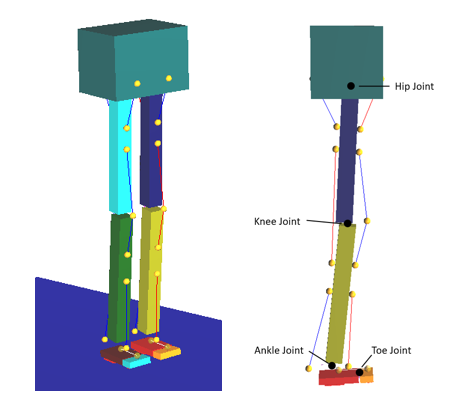
\includegraphics[width=0.64\textwidth,height=0.30\textheight,keepaspectratio]{OurWalker.png}
\par\medskip
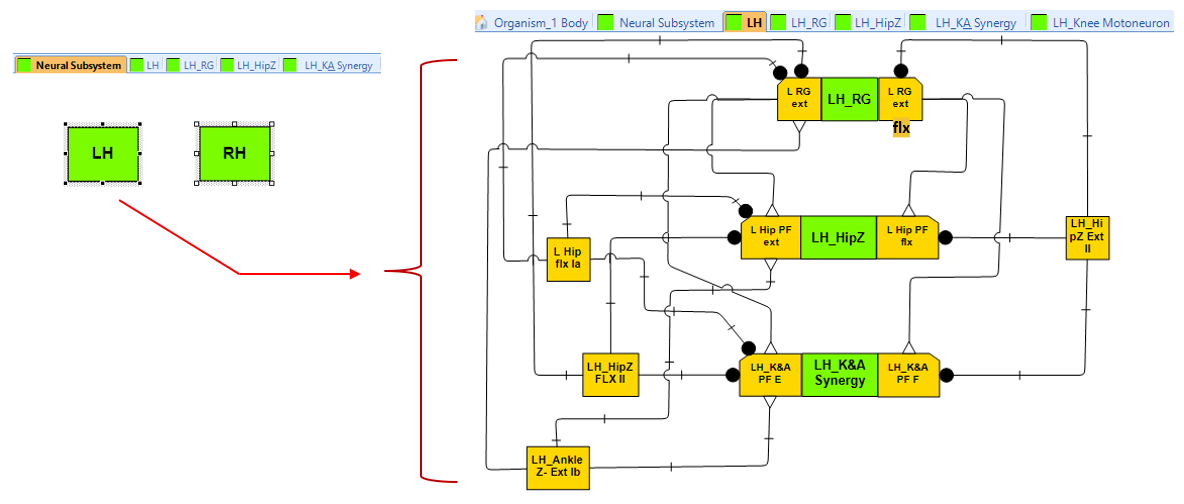
\includegraphics[width=\textwidth,height=0.31\textheight,keepaspectratio]{2layerImprove.png}
\caption[AnimatLab walker and controller hierarchy]{AnimatLab walker (top) and bilateral controller hierarchy (bottom). The model combines the Li walker mechanics and Deng CPG organization. These diagrams show construction; the suspended stepping result is described in the text.}
\label{fig:animatlab_model_architecture}
\end{figure}

\section{Requirements for the New Tools}\label{sec:sns_gaps}

The existing workflow lacked four connections needed for the BPA-actuated robot: an SNS coupled to the human-scale and BPA-routed musculoskeletal models; transferable implementations of the archived walker controllers; graphical circuit construction linked to a maintained mechanical simulator; and interfaces joining CAD-derived bodies, BPA forces, and neural commands. These requirements concerned integration for this robot project.

The software reviewed in Chapter~\ref{ch:background} supplied the individual components. OpenSim provided musculoskeletal geometry, MyoConverter translated that geometry to MuJoCo, and SNS-Toolbox provided neuron and synapse models \citep{delp_opensim_2007, caggiano_myosuite_2022, todorov_mujoco_2012, nourse_sns_2023}. Simulink provided graphical circuit construction, and Simscape Multibody provided a route for importing mechanical geometry. My contribution was to connect these components for the models and actuators used here and to establish tests of the resulting implementations. Different environments served different tasks: scripted simulation and parameter search in MuJoCo, graphical model assembly in Simulink, and reference-model evaluation in AnimatLab.

\section{Software Tools}\label{sec:preliminary_sim_methods}

The tools connect musculoskeletal geometry, actuator forces, and neural circuits. Table~\ref{tab:sns_capability} separates the implemented interfaces from incomplete mechanical integration. Figure~\ref{fig:pipeline} shows their relationship to the proposed hardware system.

\begin{table}[htbp]
\caption[Neuromechanical tools and verification scope]{Implemented tools, representative checks, and limits. A successful interface test does not establish walking performance.}
\label{tab:sns_capability}
\small
\begin{tabularx}{\textwidth}{@{}>{\raggedright\arraybackslash}p{0.23\textwidth}>{\raggedright\arraybackslash}p{0.34\textwidth}>{\raggedright\arraybackslash}X@{}}
\toprule
\textbf{Tool} & \textbf{Implemented capability} & \textbf{Verification and limit} \\
\midrule
MuJoCo--SNS coupling & Converted musculoskeletal model, BPA force interface, and afferent feedback & Actuator geometry and dynamic signs checked; supported closed-loop evaluations, not unsupported walking \\
SNS-Simscape library & Editable neuron, synapse, sensory, and actuator blocks & Reflex demonstrations and controller comparisons; generic BPA demonstration parameters remain provisional \\
Controller ports and test scripts & Comparable neural implementations and repeatable evaluations & Rhythm-core agreement across NumPy and Simulink; agreement is specific to the tested network and inputs \\
Mechanical imports & OpenSim-derived and SolidWorks-derived mechanisms in Simscape Multibody & Mechanism import achieved; the SolidWorks knee's welded joint and incomplete muscle integration remain limitations \\
\bottomrule
\end{tabularx}
\end{table}

\subsection{Model Conversion and Actuator Coupling}\label{sec:sns_existing_tools}

MyoConverter supplies the initial OpenSim-to-MuJoCo translation. I added repair and audit steps for the custom muscle paths and joint conventions, then coupled the converted model to an SNS-Toolbox controller. The converted model carries 92 muscle-tendon actuators. Geometry comparisons against the source and individual-actuator tests check that the conversion preserves the intended attachment paths and torque directions. The neural and mechanical models exchange signals at a \qty{2}{\milli\second} step.

The BPA interface evaluates the quasi-static actuator force model from Chapter~\ref{ch:muscles} using the simulated muscle length and pressure. It provides an actuator model for controller development, rather than a simulation of valve and pressure dynamics. The controller receives length, velocity, force, and contact signals through the corresponding sensory channels. The correction terms of Chapter~\ref{ch:torque} do not by themselves verify the transferred routing or compliance of a dynamic model; these require separate checks.

\subsection{Graphical Circuit Construction}\label{sec:sns_new_tools}

The SNS-Simscape library implements neuron, synapse, afferent-encoder, activation, and muscle-force elements as editable Simulink blocks. It extends the laboratory's earlier modeling approach \citep{hunt_development_2017, young_analyzing_2019} to the BPA interfaces used here. The added components connect neural signals to the actuator and mechanical interfaces. Figure~\ref{fig:simulink_sns_implementation} shows the core blocks and graded-neuron signal flow.

Two mechanical import routes were investigated. The OpenSim-derived body imports as a mechanism whose muscles must be connected through actuator blocks. The SolidWorks knee imports with its intended hinge welded because the exporter does not preserve the hinge mates. Consequently, the import is not evidence of a controlled biomimetic knee. These limits are separate from the standalone reflex demonstrations.

\begin{figure}[htbp]
\centering
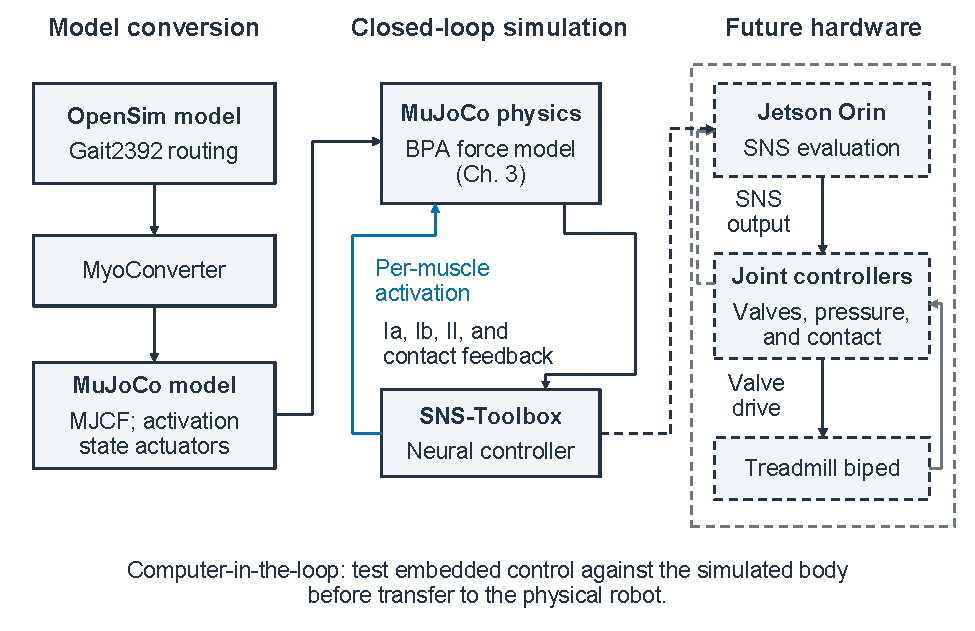
\includegraphics[width=\textwidth]{pipeline.pdf}
\caption[Simulation-to-robot pipeline]{Model conversion, closed-loop simulation, and proposed hardware deployment. Solid simulation interfaces connect neural activation to BPA force and return afferent signals. The embedded valve-control and network-evaluation system is future work (Chapter~\ref{ch:futurework}).}
\label{fig:pipeline}
\end{figure}

\begin{figure}[p]
\centering
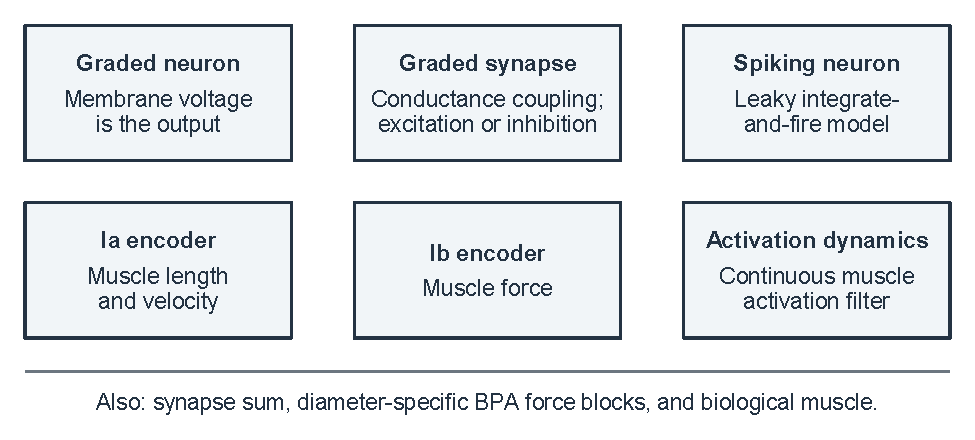
\includegraphics[width=0.94\textwidth,height=0.42\textheight,keepaspectratio]{sns_library_overview.pdf}
\par\medskip
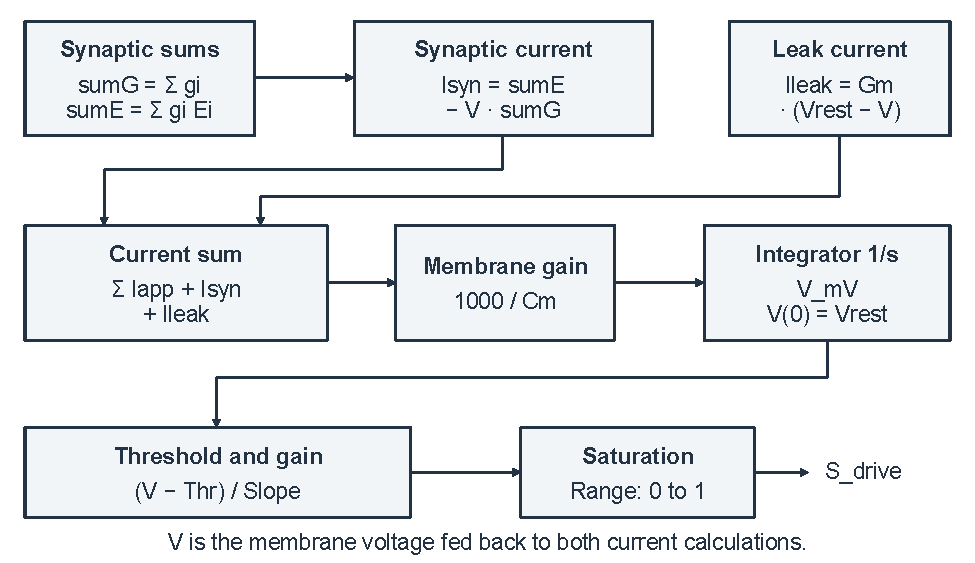
\includegraphics[width=0.94\textwidth]{simulink_neuron_detail.pdf}
\caption[Simulink SNS library blocks and neuron implementation]{Core SNS-Simscape blocks (top) and graded-neuron implementation (bottom). Summed currents drive membrane integration; threshold, inverse-slope gain, and saturation bound the output. Voltage feeds both current calculations. The generic BPA demonstration remains provisional.}
\label{fig:simulink_sns_implementation}
\end{figure}

\section{Verification of the Implemented Interfaces}\label{sec:preliminary_sim_results}

The tests address three distinct questions: whether a circuit produces its expected response, whether implementations agree under matched inputs, and whether the neural and mechanical models exchange signals in a closed loop.  The larger evaluation sets and their limitations are collected in Appendix~\ref{app:simulation_verification}; neuron equations and calibration details remain in Appendix~\ref{app:neuron_equations}.

\subsection{Reflex Response}\label{sec:sns_simulink_demos}

The library assembles Ia stretch excitation, reciprocal inhibition, and Ib autogenic inhibition in a reduced-order antagonist knee model (Figure~\ref{fig:simulink_reflex_topology}). A second demonstration tests the stretch reflex in an arm holding a beverage container as it is loaded. With the reflex enabled, arm sag was \ang{2.00}, compared with \ang{7.85} when it was disabled. The comparison checks the implemented feedback response; experimental calibration of the mechanical parameters remains necessary.

\begin{figure}[p]
\centering
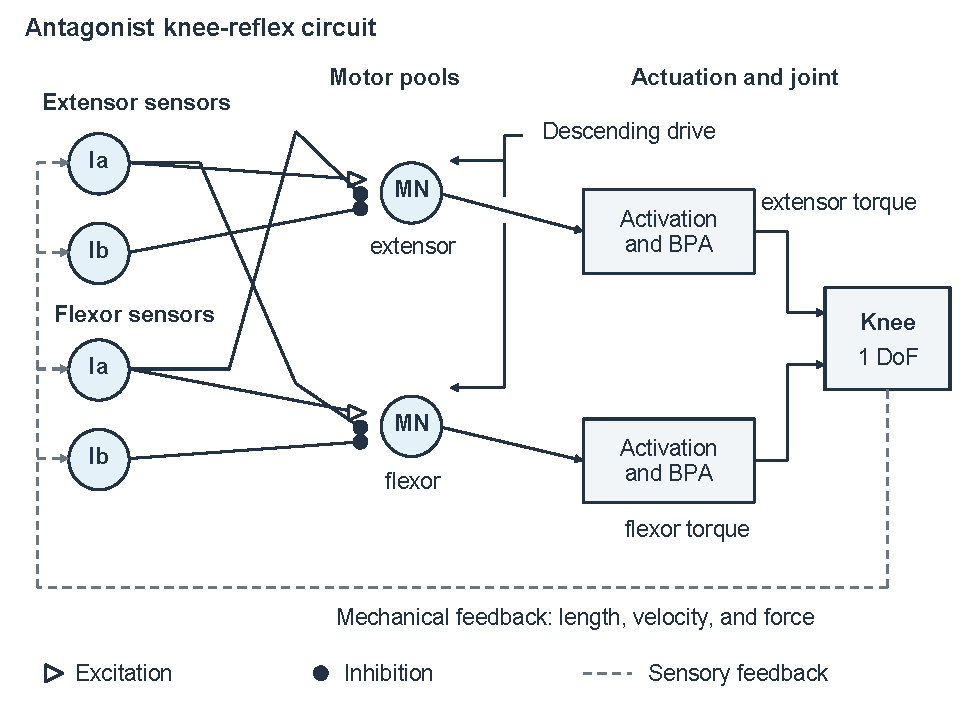
\includegraphics[width=\textwidth]{KneeReflex_circuit.pdf}
\caption[Reduced-order knee-reflex circuit topology]{Reduced-order antagonist knee-reflex circuit. Triangles mark excitation, and filled circles mark inhibition. Ia input excites the homonymous motor pool and inhibits its antagonist; Ib input inhibits the homonymous pool. Motor output drives activation and BPA-force blocks. Mechanical parameters and the generic BPA block remain provisional.}
\label{fig:simulink_reflex_topology}
\end{figure}

\subsection{Matched Neural Implementations}\label{sec:crossengine_results}

The contact-driven W2L rhythm core was implemented in NumPy and native Simulink blocks from a common connectivity specification. Both implementations received the same input protocol. Burst periods matched at \qty{1.000}{\second}, all ten expected bursts were reproduced, and voltage-trace correlation was at least 0.99996 (Figure~\ref{fig:w2l_crossengine}). The agreement is specific to this circuit and input protocol.

Removing the phasic heel-contact inputs caused the circuit to latch in both implementations. The alternating activity therefore depends on the specified sensory drive.

\begin{figure}[htbp]
\centering
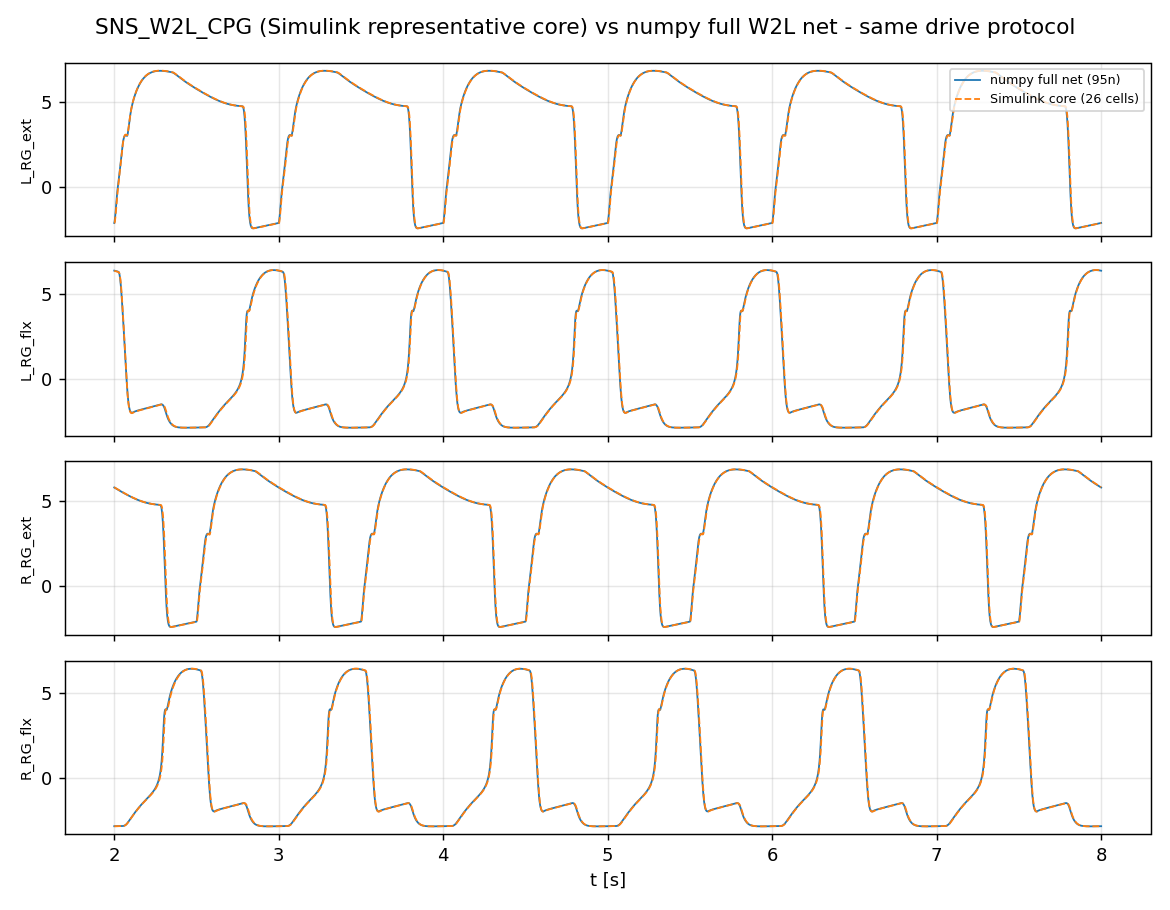
\includegraphics[width=\textwidth,height=0.55\textheight,keepaspectratio]{sns_w2l_traces.png}
\caption[W2L rhythm-core traces across engines]{W2L rhythm-generator voltages under matched inputs in NumPy and Simulink. Burst periods and counts agree; full-trace correlation is at least 0.99996. The residual \qty{2}{\milli\second} lag is one discrete solver step. The test concerns the driven rhythm core, not walking mechanics.}
\label{fig:w2l_crossengine}
\end{figure}

\subsection{Closed-Loop Model Coupling}

The MuJoCo--Simulink bridge was tested against an independent Python integration using single-muscle activation, different control rates, and sensor readback. Readback was bit-exact over the scored window. The exported neural network also drove all 92 actuators during a \qty{5}{\second} closed-loop run. Commands and measurements passed through the interface. However, under tonic drive alone the Simulink realization reached a fixed point while the NumPy reference oscillated. The network-level discrepancy remains a limit on transferring tuned controller parameters between implementations.

\section{Capabilities and Remaining Limits}\label{sec:sns_discussion}

The AnimatLab attempt motivated a repeatable way to connect neural circuits to mechanical models and test their individual interfaces. The resulting tools provide converted geometry, a BPA-force interface, graphical neural components, controller ports, and automated comparisons. The reflex and rhythm-core tests demonstrate specific circuit behaviors; the bridge tests demonstrate closed-loop signal exchange. Mechanical import, controller transfer, and locomotion performance remain separate validation problems.

The supported robot evaluations produced stepping-like motion and, in some configurations, forward progression, but no harness-free walking. Reducing tonic neural drive did not remove mechanical support. Spiking-neuron comparisons preserved a continuous motor-activation interface while changing rhythm timing and, in some runs, limb coordination (Appendix~\ref{app:simulation_verification}).

The next step is to use these interfaces and tests to improve weight-bearing control and then evaluate transfer to hardware. Chapter~\ref{ch:futurework} discusses those extensions. 
